
\chapter{Queues}
\label{chap-queue}

A Queue (pronounced by saying the first letter and ignoring all the others) is a data structure which emulates the real word functionality of standing in a line (or queue, for those from Commonwealth nations).  
In a Queue, items are processed in the order they are inserted into the Queue.  So if Alice enters the Queue, followed by Bob, followed by Carla, Alice would be the first to leave the Queue, then Bob, and then Carla.
In other words, the item that has been in the queue the longest is at the front of the Queue and is the next to be processed.


We often refer to a Stack as the LIFO data structure (I)
The use cases for Queues are fairly obvious.

\section{The Abstract Data Type}
The commans

\section{Linked Based Implementation} 
\section{Array Based Implementation}
We could use 

\section{Language Implementation}
\subsection{Java's Implementation}
\subsubsection{The \texttt{Deque}}

\subsection{Python's Implementation}

\begin{figure}
	\centering
	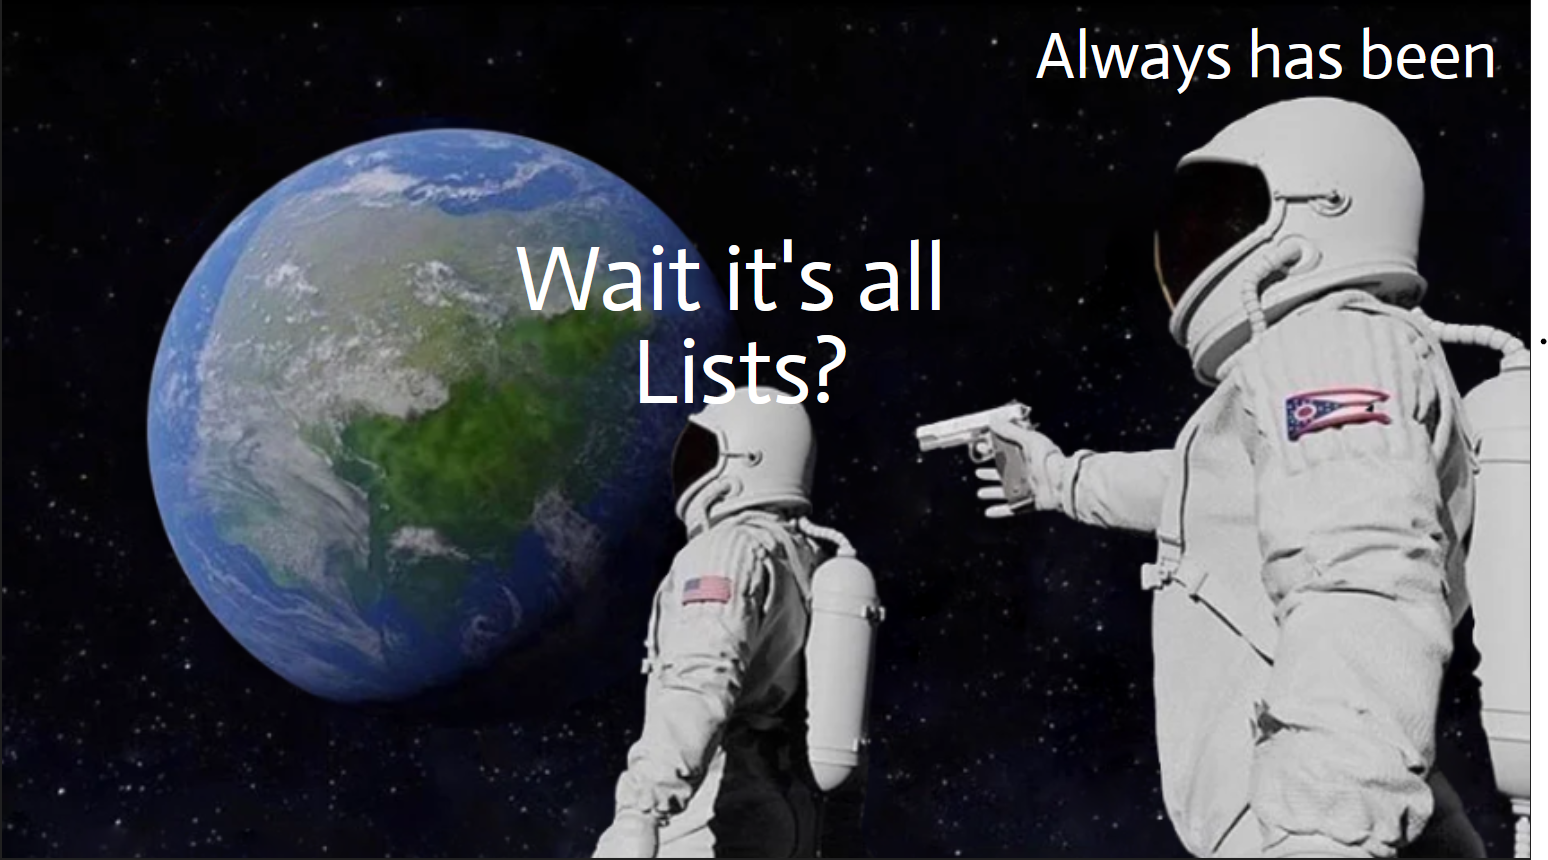
\includegraphics[width=\linewidth]{pics/waitQueuesAreLists}
	\caption{You, after learning about how to do stacks and queues in Python.}
	\label{fig:waitqueuesarelists}
\end{figure}
